\documentclass[11pt, twoside]{report}
\usepackage[utf8]{inputenc}
\usepackage{graphicx}
\usepackage{wrapfig}
\usepackage[a4paper, width=150mm, top=25mm, bottom=30mm, bindingoffset=20mm]{geometry}
\usepackage[toc,page]{appendix}
\usepackage{pdfpages}
\usepackage{natbib}
\usepackage{dirtytalk}
\usepackage{pdflscape}
\usepackage{longtable}
%\usepackage{showframe}
\usepackage{multirow}
\usepackage{textcomp}
\usepackage{fancyhdr}
\usepackage{tikz}
\usepackage{helvet}
\usepackage{hyphenat}
\usepackage{subcaption}
\usepackage{float}
\usepackage{array}
\usepackage{hyperref}
\usepackage[section]{placeins}
\renewcommand{\familydefault}{\sfdefault}
\def\checkmark{\tikz\fill[scale=0.4](0,.35) -- (.25,0) -- (1,.7) -- (.25,.15) -- cycle;} 
\pagestyle{fancy}
\fancyhf{}
\fancyhead[LE, RO]{\thepage}
\fancyhead[LO, RE]{\leftmark}
\fancyfoot[c]{Bournemouth University, Department of Computing and Informatics, Final Year Project}
\setlength{\headheight}{13.6pt}
\linespread{1.3}
\bibliographystyle{buHarvard}
\bibpunct{(}{)}{,}{a}{}{ }
\graphicspath{ {images/}{appendices/} }
\footskip = 15mm

\begin{document}
\hypersetup{
	colorlinks,
	citecolor=black,
	filecolor=black,
	linkcolor=black,
	urlcolor=black
}
\pagenumbering{roman}
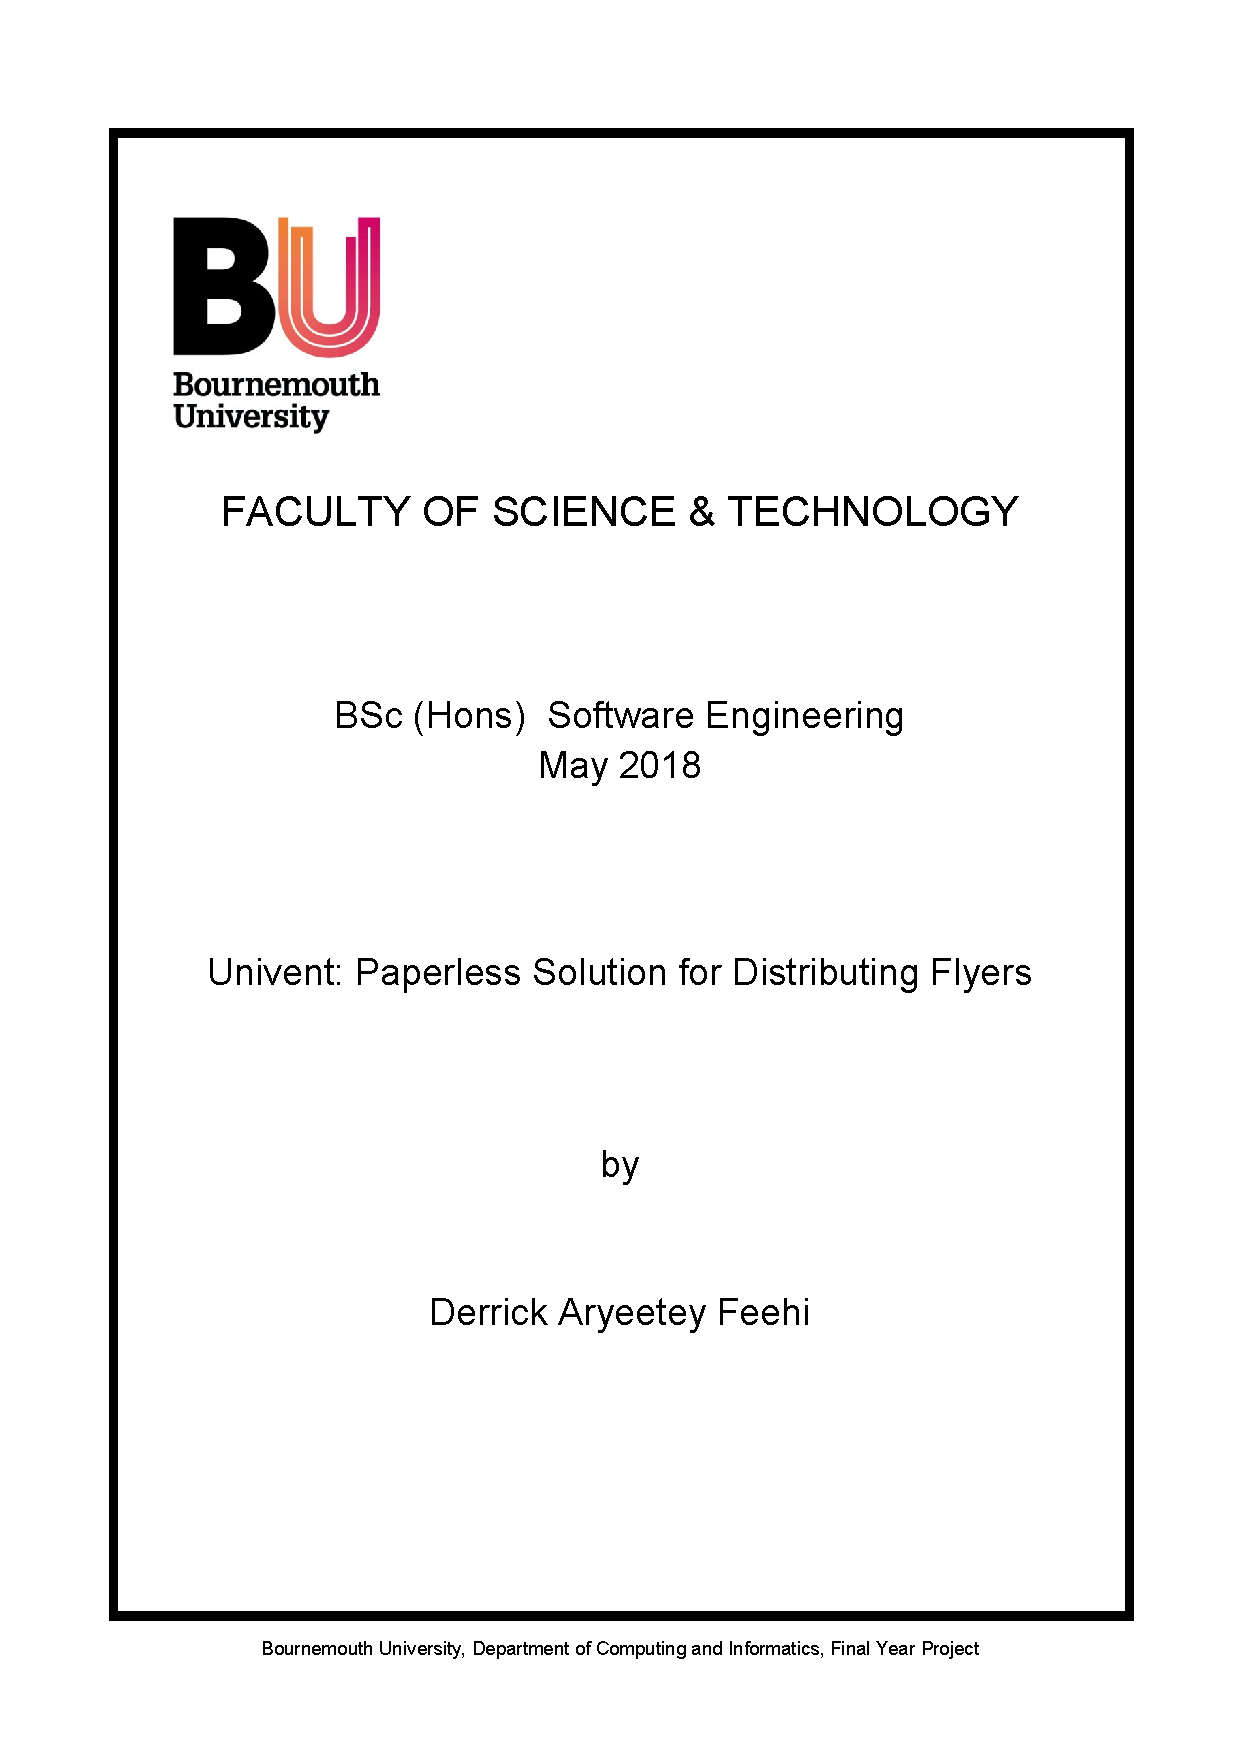
\includepdf{first_page}

\vspace*{\fill}
\begingroup
\centering
Faculty of Science \& Technology

Department of Computing and Informatics

Final Year Project

\endgroup
\vspace*{\fill}
\chapter*{Abstract}

Events are mostly published via social media; however, the main method is by distributing flyers on campus and stand advertisement. These leaflets are disregarded as they always end up in the bin, they also lack long term impact as many may read them and discard or misplace them, ending up with nothing to remind them of the event. 

Bournemouth University currently has more than 17000 students enrolled, most of these students participate and organise events every single day. Events such as seminars, talks, parties, sports etc.

There is a need for an event application to help people publish events and keep track with any upcoming events.

The app described and analysed in this thesis will address this need and assist event organisers or those interested in going to such event. This app will aid publishing the event on a platform where all student on faculty will have access to. The app will also provide attendees with all relevant information pertaining to the events they are interested in. 

The app stores users name of all those going to the event and creates a total number of those that have accepted the event, so the organisers are able to prepare accordingly. The fact that other students viewing the event can see who is attending, if students were undecided as to whether to attend, seeing their friends are attending might convince them in going.

Mobile Event apps are very common now, due to the increase of smartphones, therefore this app is very important as it provide easy access to all information that are usually required regarding an event.

This thesis describes the design, implementation of an Android app with a server side and describes the structure and what methodology and language is needed. In addition, it will also describe how this app communicates with the server database through the API and any potential security risk.
Currently this app will be for Android platform only. This app will be communicating constantly with a database server, MYSQL through an API written in PHP running on a webhost.

By providing all the benefit, and useful features of the application, it should show how essential it is to have a unique mobile platform for universities where events can be posted, minimizing effort and maximizing benefit to all attendees and event planners.

\chapter*{Dissertation Declaration}
{\linespread{1.0} %The BU template dictates this to be this line spacing
I agree that, should the University wish to retain it for reference purposes, a copy of my dissertation may be held by Bournemouth University normally for a period of 3 academic years. I understand that once the retention period has expired my dissertation will be destroyed.

\section*{Confidentiality}
I confirm that this dissertation does not contain information of a commercial or confidential nature or include personal information other than that which would normally be in the public domain unless the relevant permissions have been obtained. In particular any information which identifies a particular individual's religious or political beliefs, information relating to their health, ethnicity, criminal history or sex life has been anonymised unless permission has been granted for its publication from the person to whom it relates.

\section*{Copyright}
The copyright for this dissertation remains with me.
 
\section*{Requests for Information}
I agree that this dissertation may be made available as the result of a request for information under the Freedom of Information Act.
\\ \newline
\textbf{Signed:}
\\
Name:  Derrick Aryeetey Feehi
\\
Date: 10 May 2018
\\
Programme: BSc (Hons) Software Engineering
}

\chapter*{Original Work Declaration}

This dissertation and the project that it is based on are my own work, except where stated, in accordance with University regulations.
\\ \newline
\textbf{Signed:}

\chapter*{Acknowledgements}
First and foremost, to my supervisor Deniz Centinkaya, for the support and the constant feedback.

I would also like to thank my incomparable aunties, Deborah Quartey and Magdalene Quartey for  being there when needed. 
My sincere appreciation to my family who have been a major support throughout the entire project.

Finally I would like to thank those people who also helped me to make the project possible; Omolola Fagbule, Joshua Tubana, Gernot Liebchen and Raian Ali.


\tableofcontents

\listoffigures

\listoftables
\clearpage
\pagenumbering{arabic}

%!TEX root = ../main.tex
% What is the project about? 
% What problem are you tackling? 
% What is your research question? 
% Why do these problems need solutions? Why are they important?
% What is the background to the problem? Who is the client? What do they want?
% What existing methods have been tried? How has I.T. been applied so far? 
% What constraints do you have? (Time, PCs, money, users, software etc) 
% What is the scope of what you have set yourself to do. What is not included?
% What broad approach was taken? (Summarise your broad approach the project) 

\chapter{Introduction}
\label{chap:intro}
Lorem ipsum dolor sit amet, consectetur adipisicing elit \citep{UbuntuSecurity}, sed do eiusmod
tempor incididunt ut labore et dolore magna aliqua. Ut enim ad minim veniam,
quis nostrud exercitation ullamco laboris nisi ut aliquip ex ea commodo
consequat. Duis aute irure dolor in reprehenderit in voluptate velit esse
cillum dolore eu fugiat nulla pariatur. Excepteur sint occaecat cupidatat non
proident, sunt in culpa qui officia deserunt mollit anim id est laborum	

Lorem ipsum dolor sit amet, consectetur adipisicing elit, sed do eiusmod
tempor incididunt ut labore et dolore magna aliqua. Ut enim ad minim veniam,
quis nostrud exercitation ullamco laboris nisi ut aliquip ex ea commodo
consequat. Duis aute irure dolor in reprehenderit in voluptate velit esse
cillum dolore eu fugiat nulla pariatur. Excepteur sint occaecat cupidatat non
proident, sunt in culpa qui officia deserunt mollit anim id est laborum.

\section{Research Rationale}
Lorem ipsum dolor sit amet, consectetur adipisicing elit, sed do eiusmod
tempor incididunt ut labore et dolore magna aliqua. Ut enim ad minim veniam,
quis nostrud exercitation ullamco laboris nisi ut aliquip ex ea commodo
consequat. Duis aute irure dolor in reprehenderit in voluptate velit esse
cillum dolore eu fugiat nulla pariatur. Excepteur sint occaecat cupidatat non
proident, sunt in culpa qui officia deserunt mollit anim id est laborum.

Lorem ipsum dolor sit amet, consectetur adipisicing elit, sed do eiusmod
tempor incididunt ut labore et dolore magna aliqua. Ut enim ad minim veniam,
quis nostrud exercitation ullamco laboris nisi ut aliquip ex ea commodo
consequat. Duis aute irure dolor in reprehenderit in voluptate velit esse
cillum dolore eu fugiat nulla pariatur. Excepteur sint occaecat cupidatat non
proident, sunt in culpa qui officia deserunt mollit anim id est laborum.

Lorem ipsum dolor sit amet, consectetur adipisicing elit, sed do eiusmod
tempor incididunt ut labore et dolore magna aliqua. Ut enim ad minim veniam,
quis nostrud exercitation ullamco laboris nisi ut aliquip ex ea commodo
consequat. Duis aute irure dolor in reprehenderit in voluptate velit esse
cillum dolore eu fugiat nulla pariatur. Excepteur sint occaecat cupidatat non
proident, sunt in culpa qui officia deserunt mollit anim id est laborum.

%!TEX root = ../main.tex

\chapter{Literature Review}
\label{chap:litReview}
Lorem ipsum dolor sit amet, consectetur adipisicing elit, sed do eiusmod
tempor incididunt ut labore et dolore magna aliqua. Ut enim ad minim veniam,
quis nostrud exercitation ullamco laboris nisi ut aliquip ex ea commodo
consequat. Duis aute irure dolor in reprehenderit in voluptate velit esse
cillum dolore eu fugiat nulla pariatur. Excepteur sint occaecat cupidatat non
proident, sunt in culpa qui officia deserunt mollit anim id est laborum.

Lorem ipsum dolor sit amet, consectetur adipisicing elit, sed do eiusmod
tempor incididunt ut labore et dolore magna aliqua. Ut enim ad minim veniam,
quis nostrud exercitation ullamco laboris nisi ut aliquip ex ea commodo
consequat. Duis aute irure dolor in reprehenderit in voluptate velit esse
cillum dolore eu fugiat nulla pariatur. Excepteur sint occaecat cupidatat non
proident, sunt in culpa qui officia deserunt mollit anim id est laborum.

\begin{figure}[t]
	\centering
	
\includegraphics[width=0.45\textwidth]{unilogo.jpg}
	\caption{Bournemouth University}
	\label{fig:BULogo}
\end{figure}

Lorem ipsum dolor sit amet, consectetur adipisicing elit, sed do eiusmod
tempor incididunt ut labore et dolore magna aliqua. Ut enim ad minim veniam,
quis nostrud exercitation ullamco laboris nisi ut aliquip ex ea commodo
consequat. Duis aute irure dolor in reprehenderit in voluptate velit esse
cillum dolore eu fugiat nulla pariatur. Excepteur sint occaecat cupidatat non
proident, sunt in culpa qui officia deserunt mollit anim id est laborum.

\section{Section}
Lorem ipsum dolor sit amet, consectetur adipisicing elit, sed do eiusmod
tempor incididunt ut labore et dolore magna aliqua. Ut enim ad minim veniam,
quis nostrud exercitation ullamco laboris nisi ut aliquip ex ea commodo
consequat. Duis aute irure dolor in reprehenderit in voluptate velit esse
cillum dolore eu fugiat nulla pariatur. Excepteur sint occaecat cupidatat non
proident, sunt in culpa qui officia deserunt mollit anim id est laborum.

Lorem ipsum dolor sit amet, consectetur adipisicing elit, sed do eiusmod
tempor incididunt ut labore et dolore magna aliqua. Ut enim ad minim veniam,
quis nostrud exercitation ullamco laboris nisi ut aliquip ex ea commodo
consequat. Duis aute irure dolor in reprehenderit in voluptate velit esse
cillum dolore eu fugiat nulla pariatur. Excepteur sint occaecat cupidatat non
proident, sunt in culpa qui officia deserunt mollit anim id est laborum.

Lorem ipsum dolor sit amet, consectetur adipisicing elit, sed do eiusmod
tempor incididunt ut labore et dolore magna aliqua. Ut enim ad minim veniam,
quis nostrud exercitation ullamco laboris nisi ut aliquip ex ea commodo
consequat. Duis aute irure dolor in reprehenderit in voluptate velit esse
cillum dolore eu fugiat nulla pariatur. Excepteur sint occaecat cupidatat non
proident, sunt in culpa qui officia deserunt mollit anim id est laborum.

\subsection{Subsection}
Lorem ipsum dolor sit amet, consectetur adipisicing elit, sed do eiusmod
tempor incididunt ut labore et dolore magna aliqua. Ut enim ad minim veniam,
quis nostrud exercitation ullamco laboris nisi ut aliquip ex ea commodo
consequat. Duis aute irure dolor in reprehenderit in voluptate velit esse
cillum dolore eu fugiat nulla pariatur. Excepteur sint occaecat cupidatat non
proident, sunt in culpa qui officia deserunt mollit anim id est laborum.

Lorem ipsum dolor sit amet, consectetur adipisicing elit, sed do eiusmod
tempor incididunt ut labore et dolore magna aliqua. Ut enim ad minim veniam,
quis nostrud exercitation ullamco laboris nisi ut aliquip ex ea commodo
consequat. Duis aute irure dolor in reprehenderit in voluptate velit esse
cillum dolore eu fugiat nulla pariatur. Excepteur sint occaecat cupidatat non
proident, sunt in culpa qui officia deserunt mollit anim id est laborum.

Lorem ipsum dolor sit amet, consectetur adipisicing elit, sed do eiusmod
tempor incididunt ut labore et dolore magna aliqua. Ut enim ad minim veniam,
quis nostrud exercitation ullamco laboris nisi ut aliquip ex ea commodo
consequat. Duis aute irure dolor in reprehenderit in voluptate velit esse
cillum dolore eu fugiat nulla pariatur. Excepteur sint occaecat cupidatat non
proident, sunt in culpa qui officia deserunt mollit anim id est laborum.




%!TEX root = ../main.tex
\chapter{Methodology}
\label{chap:methodology}



%!TEX root = ../main.tex
\chapter{Background Study}
\label{background}
\section {Overview}
This section will show other areas which required further research to aid in making a concrete decision as to which technology will be used for the development of the project.
\subsection{OS}
The majority of the apps on our mobile phones are native apps, meaning they are written in languages that the platform accepts, for example swift is used to write iOS apps and java is used to write Android apps while c\# is used for most Microsoft phone apps.
Native apps are very responsive and also offer the most reliable experience to user. On the other hand an hybrid app is more similar to a web app but is installed like a native app. They are normally built with javascript, HTML, and CSS and runs in something called webview, a browser within the app. Performance wise, however, it's inferior compared to native apps. 

The project was developed as a native app, using the Android OS, this was chosen based on the fact the author has knowledge of the platform and it is the OS with the largest share on the market, \cite{WebHybri87:online}.

\subsection{Database}
MYSQL was chosen as the database for this project, mainly for its scalability and its compatibility with Java and PHP language. For this reason phpMyAdmin was used aswell as a development tool to handle database management.

\section{Development Environment}
Relying on tools to develop an app is very useful as it helps accelerate the development. For Android there are various tools which this chapter will focus on describing.
To be able to build the application a development environment, Java Development Kit(JDK) and Android SDK are required.
To develop with the SDK, Google offers a bundle, the bundle comes with an IDE and the  Android SDK.

\subsection{JDK}
Java Development Kit is the essence of any java application. As defined by the Technopedia Dictionary, \say{the JDK is a software development environment used for developing Java applications and applets. It includes the Java Runtime Environment (JRE), an interpreter/loader (java), a compiler (javac), an archiver (jar), a documentation generator (javadoc) and other tools needed in Java development}.

\subsection{SDK}
Android Software Development Kit provides a selection of tools and libraries required to build Android apps to ensure the process goes as smoothly as possible and the SDK is used to get it to run on an Android device and access unique features of the OS.

\subsection{Android Emulator}
The emulator allows to run the app without having to install the app on an actual Android device. It emulates most of the functionality of a real Android device, apart from for the
GPS module. 
\begin{figure}[h]
	\centering	
	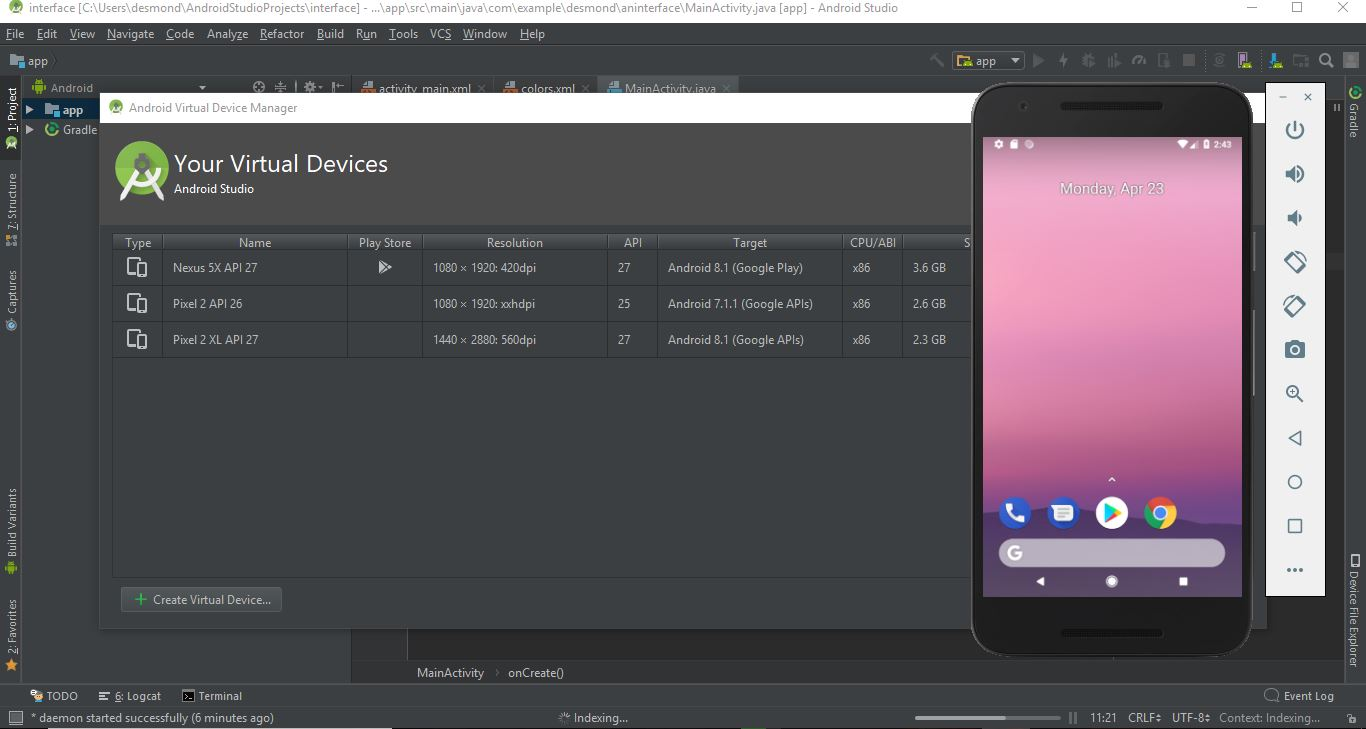
\includegraphics[width=0.5\textwidth]
	{emulator_view}
	\caption{Android Emulator}
	\label{fig:android_emulator}	
\end{figure}

\subsection{Graphic Layout}
The Layout Editor from the SDK allows developers to create user interfaces(UI) with an editor(Drag and Drop) or by writing XML Code. These editors support many features for rapid UI development and both are easy to use and it is directly included into Android Studio. The screen of the editor is shown in figure \ref{fig:android_ui_editor}.
\begin{figure}
	\centering
	\begin{subfigure}[h]{0.5\textwidth}  	      
		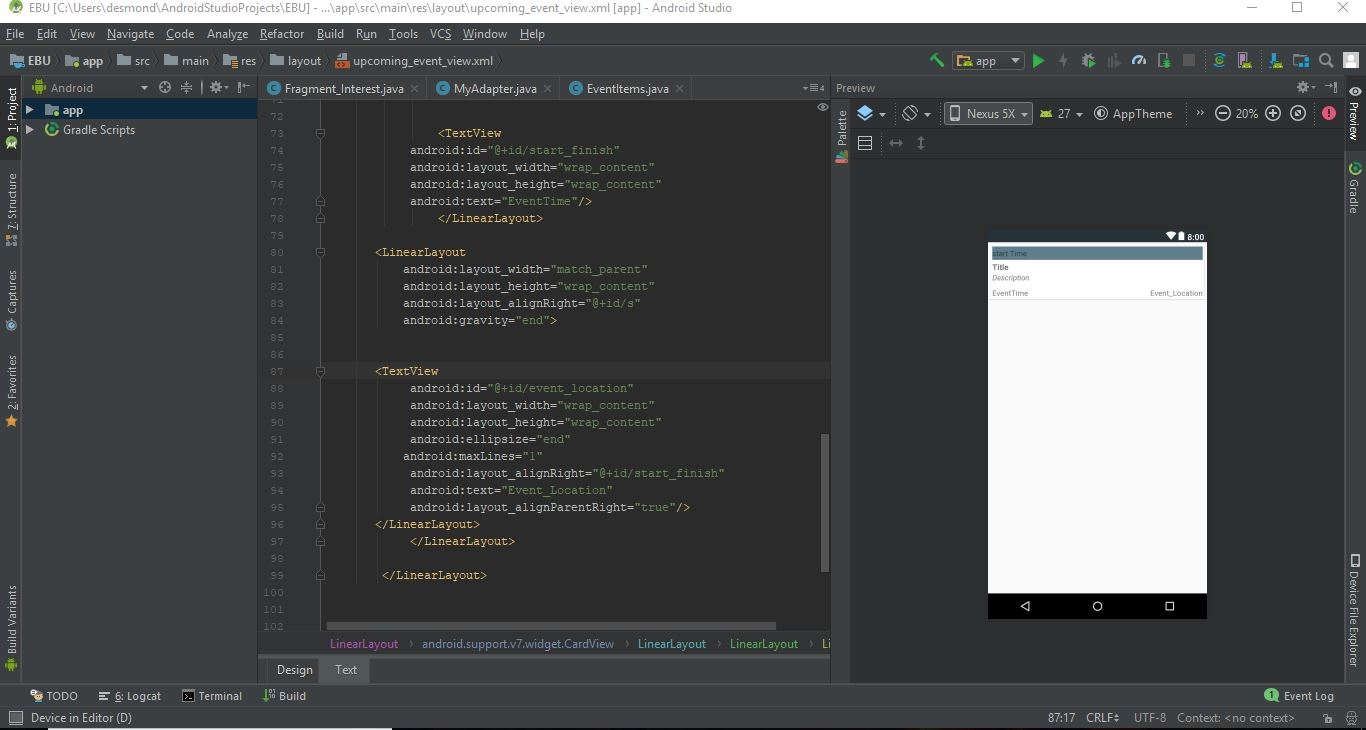
\includegraphics[width=.96\linewidth]{xml_text_view}
		\caption{XML Text View Editor}
		\label{fig:design_editor}
	\end{subfigure}%
	%add desired spacing between images, e. g. ~, \quad, \qquad etc.
	%(or a blank line to force the subfigure onto a new line)
	\begin{subfigure}[h]{0.5\textwidth}	
		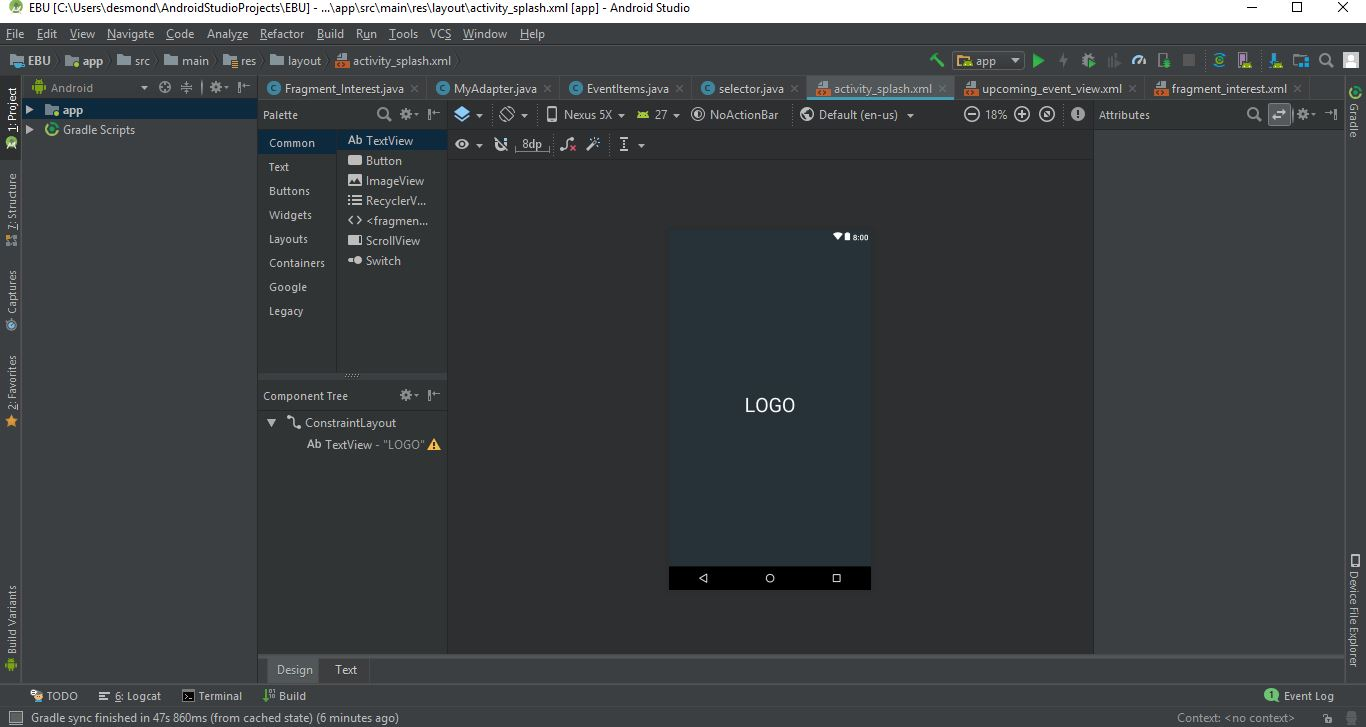
\includegraphics[width=.96\linewidth]{xml_design_view}
		\caption{XML Design View Editor}
		\label{fig:xmlEditor}
	\end{subfigure}
	\caption{Andriod UI Design Editor}\label{fig:android_ui_editor}
\end{figure}

\subsection{IDE}
According to TechTarget Integrated Development Enviroment(IDE) is \say{a software suit that consolidates the basic tool developers needs to write and test software. An IDE consists of a code editor, a compiler or interpreter and a debugger that the developer can access through a single graphical user interface}.
For the purpose of this project Android studio was used as its the official IDE for Android development.

\section {Android Framework and API}
In order to build the artefact, it is essential for the author to understand the Android framework and API, this information is found in Appendix \ref{framework}.


\section{Developing Problem}
Dealing with diverse platform is on of the most challenging aspect in app development. Mobile development is moving towards fragmentation rather than unification.

\textbf{Fragmentation:} Considering Android devices, most of them comes with different screen resolution. Different devices exist with different properties such as  CPU speed and memory. According to a study made by Mona, Ali and Phillipe in their article “Real Challenges in Mobile app Development”; 76\% of their survey participants see the existence of multiple platform as a challenge for developing mobile apps, while 23\% believe it is an opportunity for technology advances that drive innovation. The development process cannot leverage knowledge from a platform to another. Also, when an application is created for various platforms, the developers must treat the development independently  and check that consistency is kept across each one.


%!TEX root = ../main.tex
\chapter{Discussion}


%!TEX root = ../main.tex
\chapter{Univent Design}
\label{chap:design}
\section{Overview}

The app design is a very important phase of the development lifecycle, as it can have an impact whether or not the app is accepted by the users. This chapter presents the choices made for the design of the aplication.

\section{Android Application Design}
\label{android app design}
The user interface is designed using widgets. Android provides  basic widgets such as, image view, textview, etc., which can be used to create the application. All these widgets are incuded in the Android SDK. Android gives users the possibility to create their own widgets, named custom widgets.

All the screens in the project are composed of various widgets, both basic and customized. 

The home screen, includes widgets such as, RecycleView, TextView, ImageView. The recycleview is populated with data directly from the database.
\begin{itemize}
	\item \textbf{TextView} - 
	A textview displays text to the user, normally displaying contextual information or the name of other elements on the screen. Figure \ref{fib:textview}, shows how to define a text view in the XML editor.	
\begin{figure}[!htbp]
		\centering
		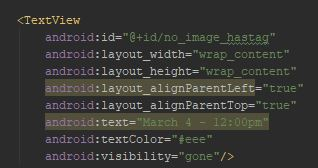
\includegraphics[width=0.23\textheight]{textview}	
		\caption{Define a TextView in XML}
		\label{fib:textview}
\end{figure}

\item \textbf{ImageView} - 
 	An Imageview is used to display image to the user from the resource file or from an external source, like the internet.	
 	The following snippet is an example of imageview, refer to figure \ref{fib:imageview}
 	
\begin{figure}[h]
 				\centering
 		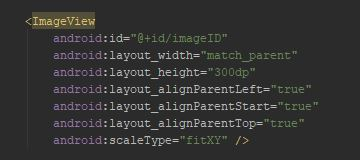
\includegraphics[width=0.45\textheight]{imageview}	
 		\caption{Define a ImageView in XML}
 		\label{fib:imageview}
\end{figure}
 \item \textbf{RecycleView} - 
According to the official android website, \say{a Recycleview is a view group that displays a list of scrollable items}. The list items are automatically inserted to the list using an Adapter that pulls content from a source such as an array or database query and converts each item result into a view that's placed into the list.
Figure \ref{fig:xmlrecycleview}, shows how to declare a recycle view.
\begin{figure}[h]
	\centering       
		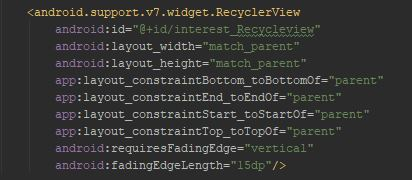
\includegraphics[width=0.45\textheight,natwidth=610,natheight=300]{recycleview}
		\caption{Defining RecycleView}
		\label{fig:xmlrecycleview}	
\end{figure} 

Recycleviews are normally accompanied with cardveiws, these shows information inside cards, and its corners can be customized by the user. The main function of these cards is to act as the rows of the recycleview.
	
\item \textbf{ViewPager - } 
A viewPager is viewgroup that allows the user to swipe left or right to display a new screen. Its a more efficient and user friendly way of displaying screens to users, refer to Appendix \ref{screen_design}.
\end{itemize} 
\pagebreak
\section{Initial Design}
Before the final design of the app was created, various designs were made in attempt to give a better UI experience to the user, refer to Appendix \ref{screen_design}. All the designs were made with the Android XML editor to see exactly how it will look on a mobile device. Using the XML editor made designing simple, meaning no need of wireframe designs before recreating them for the app, which saved a lot of time. All the widgets mentioned above in section \ref{android app design}, were used to complete the design.
Extensive research on similar applications, section \ref{similar_app}, provided inspiration for the final look of the app and the meeting with the client also provided ideas for new features to implement. 
The app was further redesigned to be more user friendly, with two new screens created, Discover and Interest(named as "for you" in the app), using viewpager, as detailed in \ref{android app design}, so users can swipe left or right to move between  screens as shown below in figure \ref{fig:homescreen}.

\begin{figure}[h]
	\centering       
	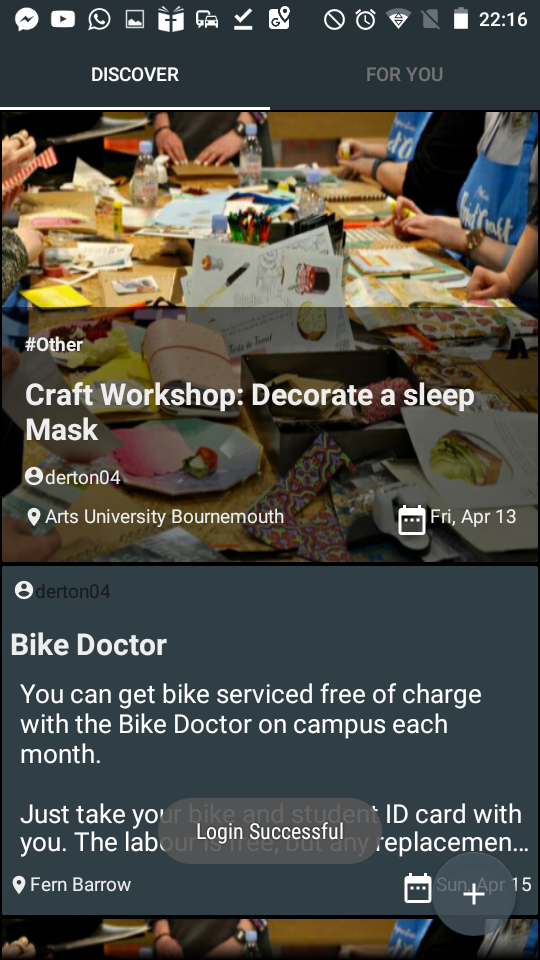
\includegraphics[width=0.25\textheight]{discover}
	\caption{Home Screen}
	\label{fig:homescreen}	
\end{figure}

The discover screen shows all the upcoming events with no filter, while the "for you" screen  shows only recommended events based on the user interest. In order to achieve this a new feature was to be added, as a way for the user to choose what they were into. A snippet of the Interest screen can be found in Appendix \ref{screen_design}.

\section{Database Design}
Figure \ref{fig:database_design}, describes the structure of the database. The event table contains all the information of the event, the user table has all the user information and finally the GoingTable, contains the ID of the users an the specific event ID the wish to attend.
\begin{figure}[h!]
	\centering       
	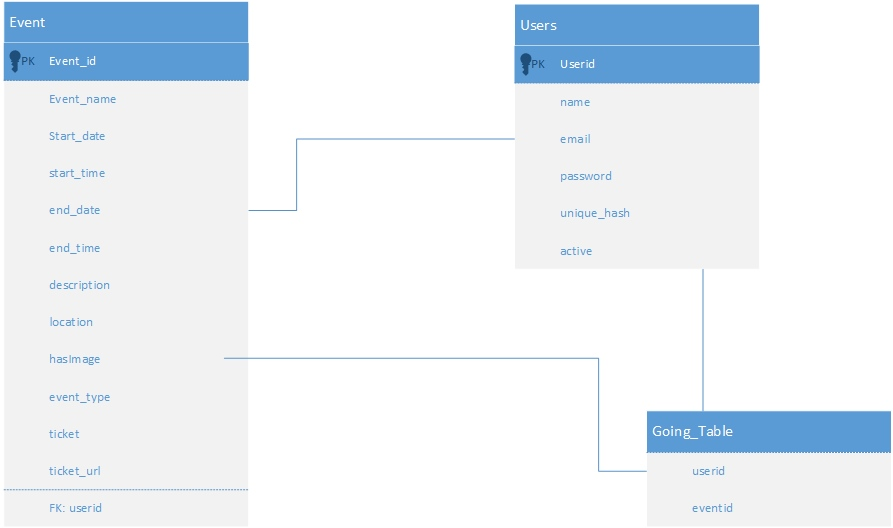
\includegraphics[width=0.6\textheight]{database_design}
	\caption{Database Design}
	\label{fig:database_design}	
\end{figure}
\subsection{Security}
 Considering the importance of data it is not a surprise for attackers to target the data these are containing. In this section various challenges in database security are discussed.
\begin{itemize}	
\item 	\textbf{Blank Password, blank email:} In order to avoid this issue, a password and email validation has been put in place, which will notify the user if any of the fields are left blank.

\item 	\textbf{Secure credential:} User passwords are not stored directly onto the database, but are encrypted using a  hash key. The hash key is then stored in the database, whenever the password is called it is then decoded.
	
\item 	\textbf{Excessive privileges:} Granting  Users (or applications) database privileges that exceed the requirements of their task, these privileges may be abused for malicious actions. 
	
\item 	\textbf{Weak Authentication:} Weak authentication allows attackers to take the identity of database users. A counter measure for this issue will be to Implement a two-factor authentication.
\end{itemize}

\subsection{General Architecture }
An Android device with the Univent application already installed communicates with the web service using a RESTful API.
The application sends HTTP requests with GET/POST method headers and receives formatted JSON responses. The API is written in PHP and handles querying the MYSQL database. Figure \ref{fig:API_design}, shows the system architecture.
\begin{figure}[h!]
	\centering       
	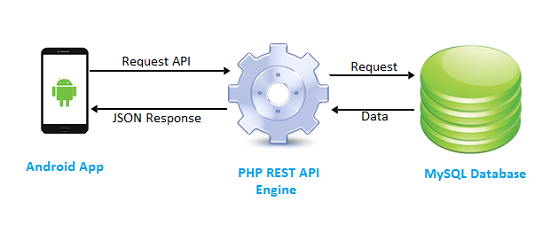
\includegraphics[width=0.5\textheight]{php-mysql-rest-api-for-android}
	\caption{Rest API}
	\label{fig:API_design}	
\end{figure}
\FloatBarrier






%!TEX root = ../main.tex
\chapter{Implementation}
\section{Overview}
This section will describe how the features were implemented to develop the final artefact, the system will be developed using Android studio. 

\begin{figure}[h!]
	\centering       
	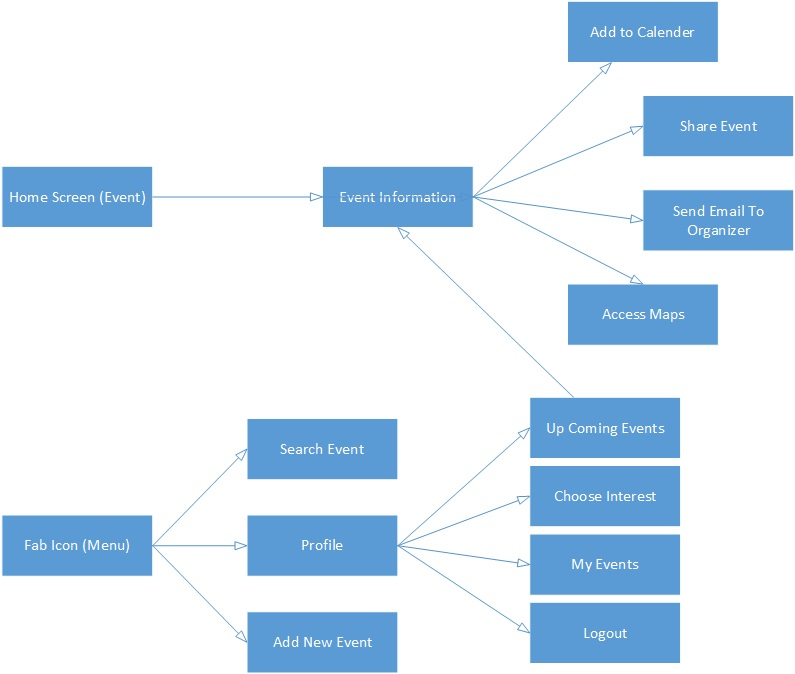
\includegraphics[width=0.35\textheight]{navigation_screens}
	\caption{Logic Flow of Screen}
	\label{fig:navigation_screen}	
\end{figure}
The figure above \ref{fig:navigation_screen} shows the relationship between each activity(screen), how to move between screens.
Both screens, upcoming event and homescreen link back to event information, because this option is available from both activities, meaning the user can access event information from both.
Add to calender, share event, send email to organizer and access maps are all behind event information, this means the logic behind each of those activities has to be implemented in the event information activity.
Fab icon, refer to figure \ref{fig:fab_menu}, is a navigation menu that links to search event, profile and add new event.
\begin{figure}
	\centering
	\begin{subfigure}[b!]{0.25\textwidth}  	      
		
\includegraphics[width=.96\linewidth]{fab_menu_not_clicked}
		\caption{Fab Not Clicked}
		\label{fig:fab_not_clicked}
	\end{subfigure}%
	%add desired spacing between images, e. g. ~, \quad, \qquad etc.
	%(or a blank line to force the subfigure onto a new line)
	\begin{subfigure}[b!]{0.25\textwidth}	
		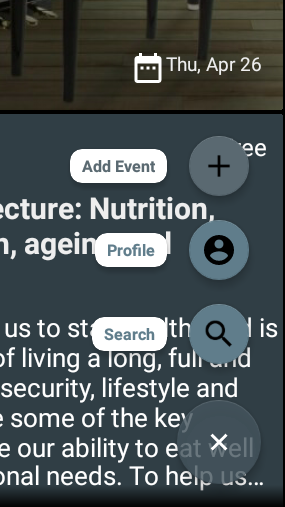
\includegraphics[width=.96\linewidth]{fab_menu_clicked}
		\caption{Fab Clicked}
		\label{fig:xml_editor}
	\end{subfigure}
	\caption{Fab Menu}\label{fig:fab_menu}
\end{figure}

\section{Login \& Register}
The login.xml has the function to display the views to the user while the login activity has the function to handle all the java logic in the background. This activity will ask the user to login, user then has to select their university, enter university email and password, this information is then checked against the user database; if the user has already got an account and the password is correct the user will be logged in successfully. This activity also checks if the user account is verified or not and displays the appropriate message. The user can move from the login activity to the Register activity by clicking on the textview, "not registered". Refer to appendix \ref{screen_design}, for details on screen design.

Activities relies on intent, refer to Appendix \ref{additional_components}, to move from one activity to the other, the figure below \ref{fig:intent} shows an example of how to move from the login activity to the register activity. Intent also allows data passage between activities; for the purposes of this app data such as user email, user ID, was passed through activities to maintain traceability.
\begin{figure}[h!]
	\centering       
	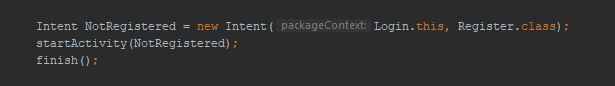
\includegraphics[width=0.5\textheight]{login_to_register}
	\caption{Declaring an Intent}
	\label{fig:intent}	
\end{figure}
In order to enhance the user experience, shared preferences APIs was used to store user login details on their phone(internal memory of the phone). Shared preferences permits saving and retrieving key value pair data to be used to save primitive data type such as Boolean, string, int, long and float.

\textbf{MODE\_PRIVATE} – this is the most used mode of sharedPreferences, It is a default mode, which means that when any preference file is created it will only be accessible from the application.

Calling the edit() function of SharedPreferences class which returns Editor class object allows to save data into sharePreferences, refer to figure \ref{fig:save_share_preferences}

\begin{figure}[h!]
	\centering       
	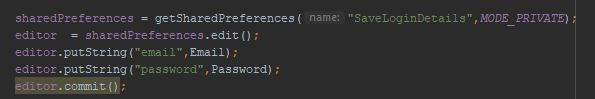
\includegraphics[width=0.5\textheight]{save_sharepreferences}
	\caption{Declaring SharePreferences}
	\label{fig:save_share_preferences}	
\end{figure}

Values stored in shared preferences can be called using SharedPreferences object by calling different primitive type function starting with get plus the Primitive type name, refer to figure \ref{fig:get_share_preferences}
\begin{figure}[h!]
	\centering       
	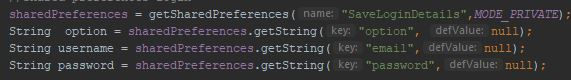
\includegraphics[width=0.5\textheight]{get_sharedpreferences}
	\caption{SharePreferences key value pair data}
	\label{fig:get_share_preferences}	
\end{figure} 
 
 The \textbf{register activity}  allows the user to create an account if they are not previously registered. It prompts the user to enter their details, university name, nickname, email and password. Afterwards, before registering the user, it verifies if the user does not have a previous account, if so it will displays a message. Otherwise it creates an account and sends a verification email to the users email address to verify their account, refer to appendix \ref{screen_design}.
 
 Once the user is registered and logged in, the app receives all the event data from the server and displays it on the home screen.

\section{Implementation of REST API}
REST stands for "Representational State Transfer" REST architecture will be used to build the client/server applications. It's simple to implement REST as it basically works on HTTP protocol, refer to figure \ref{fig:http_methods} below.
\begin{figure}[h!]
	\centering       
	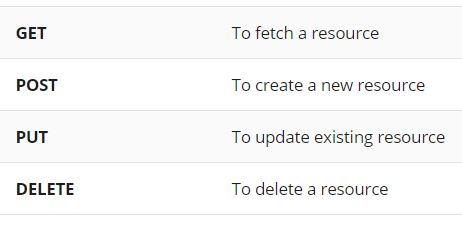
\includegraphics[width=0.5\textheight]{http_methods}
	\caption{HTTP Methods}
	\label{fig:http_methods}	
\end{figure} 

Since Android does not have a dedicated library for implementing A REST API, it provides a number of pre-implemented solutions that can be used for the implementation. According to \cite{kwon2016design}, the main issue however, is how to design an action
flow between components of the system from the presentation layer (Activities) down to the network and local memory operations.
He also mentions that there is nothing like the best way of implementing a RESTful API client on Android platform
because each solution can, and should be modified according to the unique requirements
of the protocol, however, there is one pattern which is definitely not advised, that is to, avoid running RESTful methods directly from the UI thread.
\begin{itemize}
	\item this would cause and ANR (Application Not Responding error). 
	\item slow down the application and make it less responsive 
\end{itemize}  

 Android however provides a solution, AsyncTask, which is a high-level concurrent construct. AsyncTask can interact with the UI thread by updating the UI via event handlers. For example, the event handler \textbf{\textit{onPostExecute}} executes after the task is finished, and can update the UI with the task results.
 A study by, \cite{7372076}, shows AsyncTask is the most used async construct in Android. However, it is designed for short-running tasks (i.e., less than one second) and if improperly used, can lead to memory leaks and lost results.
 
 The basic methods used in an android AsyncTask class are defined in the table below:
 
 
\begin{longtable}{| L{5cm} | L{9cm} |}
	Method  & Function  \\ \hline
doInBackground() & This method contains the code which will be executed in the background\\	\hline
	onPreExecute() &	This method contains the code which will be executed before the \textbf{\textit{doInBackground}} method\\	\hline
onProgressUpdate()   &This method receives progress updates from \textbf{\textit{doInBackground}} method\\	\hline
onPostExecute()  &	 This method is executed after \textbf{\textit{doInBackground}} completes processing and the result from \textbf{\textit{doInBackground}} is passed to this method\\	\hline
	\caption{AsynTask Methods}
	\label{methods}
\end{longtable}
\pagebreak
\subsection{Sending Request to the Server}
There are multiple networking libraries and classes available for Android that can send POST requests, however, the preferred method is through HttpUrlConnection.
This section will describe how to send request from Android client to the server;

\textbf{Giving Permission to Android:}
Univent requires an internet connection in order to get information about the event and to retrieve data from the database. All required permissions must be declared in the AndroidManifest.xml file.
\begin{figure}[h!]
	\centering       
	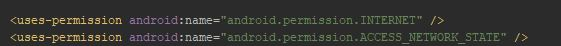
\includegraphics[width=0.5\textheight]{permission_internet}
	\caption{Internet Permission}
	\label{fig:internet_permission}	
\end{figure} 

\textbf{Connecting to the Server using URL:} The URL object, refer to figure \ref{fig:urlObject}, contains all the necessary information to reach the destination resource. In this example, the url is pointing to the php file on the server, named get\_event.php. This file handles the query to get all events from the database.
URLs are constructed as sets of information. Lets consider the URL:
\begin{center}
\textbf{ http://derton04.000webhostapp.com/login.php?parameter=value}
\end{center}

In the example above, http is the protocol, derton04.000webhostapp.com is the domain name, and login.php the path. Parameter a query parameter key (called key), value a query parameter value (named as value), and parameter=value a query parameter key-value pair (referred to as key-value pair).
\begin{figure}[h!]
	\centering       
	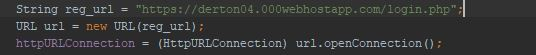
\includegraphics[width=0.5\textheight]{URL_GET_DATA}
	\caption{URL to get all Events in the Database}
	\label{fig:urlObject}	
\end{figure} 
 
 In the next step, \ref{fig:url_get}, the methods and properties of the request object are set. First, set the method as request method to be invoked as POST. The method setDoOutput, needs to be set to true before sending a post request. setDoOutput is not needed for GET requests.
  \begin{figure}[h!]
 	\centering       
 	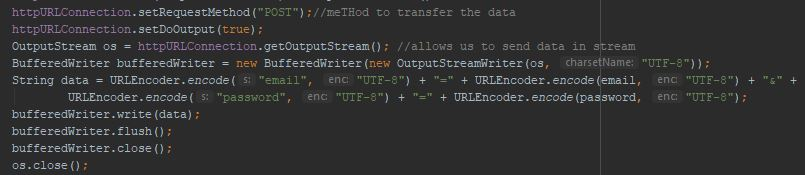
\includegraphics[width=0.5\textheight]{url_object}
 	\caption{URL to get all Events in the Database}
 	\label{fig:url_get}	
 \end{figure} 

 This library also gives the possibility of including data in the request. The URLConnection class provides an OutputStream object as the mechanism for providing this data, for performances reason it is wrapped in a buffered writer.
 The parameters/data are then attached to the url, then encoded onto the outPutStream before being transmitted over the internet.

The snippet below, figure \ref{fig:response_code} checks if the connection was successful and if the data has been transmitted.
\begin{figure}[h!]
	\centering       
	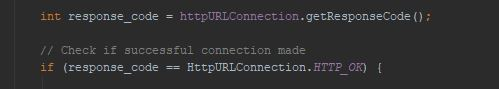
\includegraphics[width=0.4\textheight]{response_code}
	\caption{Check if Connection is OK}
	\label{fig:response_code}	
\end{figure}

 The figure below, \ref{fig:status_code}shows the status code of an http connection.
\begin{figure}[h!]
	\centering       
	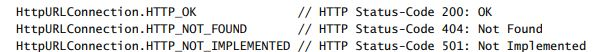
\includegraphics[width=0.4\textheight]{status_code}
	\caption{Status Code}
	\label{fig:status_code}	
\end{figure} 

 After receiving the Http status code OK, the URL will return some values that are directly coming from the database. Using inputStream and the String builder class, will fetch this data(JSON format) and store it in the variable, in this case result.
\begin{figure}[h!]
	\centering       
	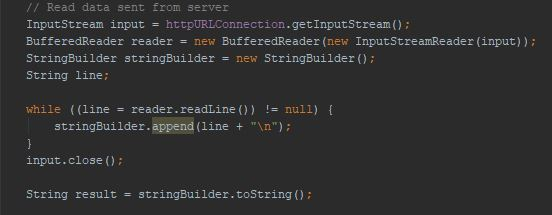
\includegraphics[width=0.4\textheight]{read_result_from_api}
	\caption{Status Code}
	\label{fig:read_result}	
\end{figure}

Figure \ref{fig:parse_json}, shows how the data is parsed using JSON parsing technique inside android application and then set into recycleview. 
\begin{figure}[h!]
	\centering       
	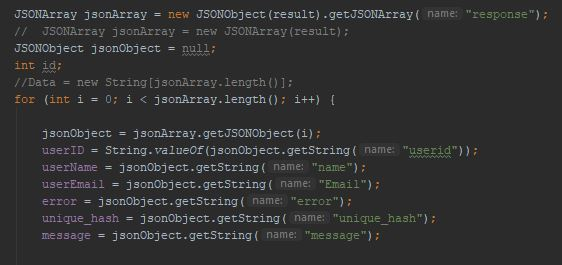
\includegraphics[width=0.4\textheight]{get_json}
	\caption{Parsing JSON}
	\label{fig:parse_json}	
\end{figure}
\pagebreak
To access the database, it requires an interface, first, it must receive JSON data, add data and update the database, secondly, it
must deliver JSON data containing events in the database.
A PHP scripts is used to provide this interface, below is a complete example of connecting an android application with MYSQL database via PHP script. It creates a basic application that retrieves data from MYSQL database using GET and POST method.

The PHP page given below takes parameters(userid) by POST method, and displays all event in the database created by that userID. The result will be displayed in JSON format.
\begin{figure}[h!]
	\centering       
	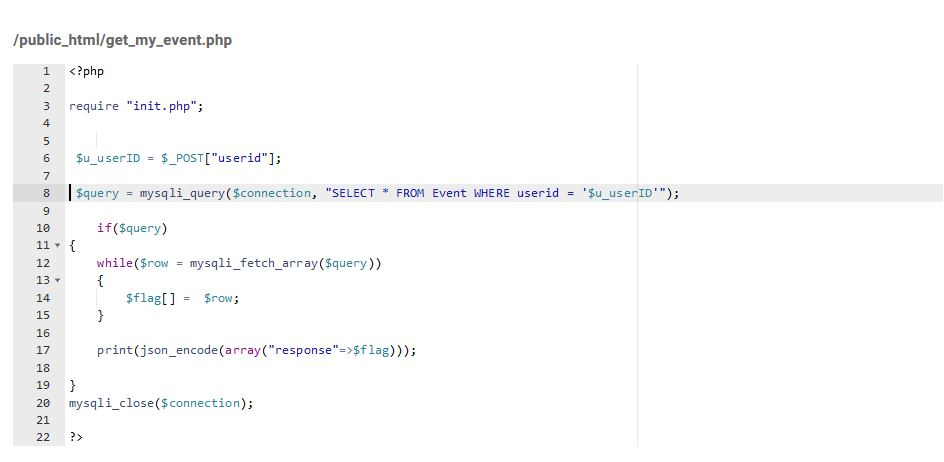
\includegraphics[width=0.5\textheight]{php_code}
	\caption{PHP Page}
	\label{fig:php_code}	
\end{figure}
The PHP file is responsible for handling the communication with the database, to insert, update, retrieve and delete data. To do so, the query is embedded in the PHP file which is then capable of establishing the connection with the MySQL database and execute the required query.

\textbf{JSON -}
JSON (JavaScript Object Notation)  is a lightweight text-data interchange format used to transmit data in form of objects(structured data: key value pairs) over the internet. JSON also supports string, Boolean, number, array and null formats for storing data.
After the database operation is done, the server will save the result as JSON format, and send it to the requesting client, refer to Appendix \ref{json} for an example of JSON data format.

\section{Sending Image to Server}
\label{sending_image_server}
This section explains how the images  of each event were uploaded to the server using the Volley library, see Appendix \ref{sending_image_server_appendix}.

\section{Testing}
To ensure the system was tested thoroughly a test suit was designed.
Test results are shown is Appendix \ref{appendix:test_suit}.
\subsection{System Testing}
The purpose of system testing is to test Univent against the functional requirements declared in section \ref{req_analysis}.
Appendix \ref{appendix:test_suit} detail the system testing.

\subsection{Black Box Testing}
Android app must be tested on the emulators, but it is important to test the app in the real world. The app has been constantly been tested from initial installation to daily use of app as per the end users point of view. This method is more powerful to come to know if any issues become visible in Android apps, as issues will surface in day to day use.

After each new functionality added, a thorough testing is done by the author, the supervisor and some experimental users. 
This method resulted in being very effective as some defects, with varying severity, were identified, for example, the send email button in the event information page, was meant to send an email to the event host, instead it was sending the email to the actual user. 
Another behaviour identified that was very crucial, was the login validation, user were allowed to register with a blank password, therefore they could login  without typing in the password. 

\section{Publishing to Play Store}
After all testing has been completed, the application was
published on the Google Play Store. 
The app was released on the Android Market under the name Univent and it will be free for all users. 

%!TEX root = ../main.tex
\chapter{Evaluation}
\section{Overview}
As usability is quite crucial for the success of the application, a random  selection of users were offered to try the application. Once they had tested the app they were asked to leave a review on the play store and fill out a survey.
Below is the outcome of the survey and some of the reviews.

\begin{longtable}{| L{7cm} | L{7cm} |}
	Question & Score  \\ \hline
	How would you rate the mobile app? & Weighted average is 4.75 out of 5 stars \\	\hline
	I found the system really easy to use &	75\% Strongly agree, 25\% Agree  \\ \hline
	I would need assistance to be able to use the app.   &	50\% neither agree or disagree, 25\% diasagree and the other 25\% strongly disagree  \\ \hline
How visually appealing is the app?  &50\% Extremely appealing, 25\% Very appealing and the other 25\% Somewhat appealing \\	\hline
I think I would use the app frequently  & 75\% agree and 25\% strongly agree \\	\hline

How likely is it that you would recommend the app to a friend or colleague?  & 50\% Extremely likely and 50\% very likely\\	\hline

Do you have any other comments about how we can improve the app?  &	see table \ref{comments}\\	\hline	\caption{Survey}
	\label{survey}
\end{longtable}
\pagebreak
\begin{longtable}{| L{6cm} | L{6cm} |}
	User & Comments  \\ \hline
	User 1  &	Good app, allows you to view events from Bournemouth University, allows you to add your own events, simple to use nice layout\\	\hline
		User 2  &	Very good app, simple user friendly interface \\	\hline
		User3  &	Create a version compatible with apple iPhones  \\	\hline
			User 4  &	Some usability issues when you verify your email address, I had to re enter Bournemouth University before i could sign in, I didnt know I had to do that without guidance  \\	\hline
			User 5  &	Pretty good app. Perfect for checking available BU uni events - convenient use. Layout is nice and simple. Good simple app \\	\hline
		\caption{User Comments}
		\label{comments}
\end{longtable}	

For general feedback, refer to table \ref{survey} and \ref{comments}. The screen design received very good feedback; the participants noticed how the screens were appealing and they also noticed how useful the artefact could be.

\subsection{Requirements Evaluation}
In terms of functionality all the requirements mentioned in chapter \ref{req_analysis} have been met.

\begin{longtable}{|  L{10cm} | c |}
	\hline
	  Requirements\newline & Met? 
	  
	  \newline Yes/No
	   \\	
	\hline
	 The application should have a register and login screen & Yes  \\
	\hline
	 The application should integrate a validation for email, only \newline Universities email are accepted & Yes  \\
	\hline
	 The application should provide specific information such as event location, event start and end date, description, title. & Yes  \\
	\hline
	 The application should provide information of all attendees interested in an activity or event  & Yes \\
	\hline
	 The application should have a \say{Share} feature. This will open any related app installed on the users phone so they can share the event with friends & Yes  \\
	\hline
	 The application should provide a \say{Send Email} feature. This will open any email client installed on users phone, so they can email the event host for further information regarding the event & Yes  \\
	\hline
	 The application should have a \say{Map Feature}. This will direct the user to the Maps application with the event location already pre entered.  & Yes \\
	\hline
	 The application should have an \say{Add to Calendar} feature. This will open any calender application on the users phone and it will allow one to save the event on the calender creating a future reminder. & Yes  \\
	\hline
	 The application should allow the user to choose the category they are most interested in and based on that information display all types of event or activities in those categories & Yes \\
	\hline
	  The application should save the user login details, so user is only required to login once. & Yes \\
	\hline
	The application should show the location on a map directly on the screen of the app  & Yes \\
	\hline
	%	\end{tabular}}
	\caption{Requirements Evaluation}
	\label{table:req_eval}
\end{longtable}	

\section{Success Criteria}
The aim of this thesis was to provide support in publishing and keeping track with activities in the faculty.
The success criteria set in section \ref{success_criteria}, has been successfully met and all requirements have been implemented.

The app was built using Android studio, the Android framework and API were discussed in chapter \ref{background}, that knowledge aid in implementing the app successfully. 
 
Overall this project was successful, all feedback regarding the system received from various users indicates users were able to use the app successfully and were able to create an event as well as keep track of any other activities posted on the app.

%!TEX root = ../main.tex
\chapter{Conclusion}
\section{Summary}
The artefact delivers exactly what it is was built for, which was to build an android app that encourages users to use the app as a platform to share events. A server side was created as a way to communicate between server and client, on the client side HttpUrlConnection and Volley were used to retrieve and send data to the server. Both solutions were adopted because of their efficiency  and simplicity in being implemented, ignoring other existing solutions like okhttp and retrofit.

The app allows users to publish their own events and view any other upcoming events on the campus. This makes publishing very easy for users, and individuals can find all information needed about an event on the go. 

The feedback received from users was very positive, and majority of them will definitely consider using the App in their daily life. 

This project will contribute in going paperless. Which will ensure cost savings for the University and will enable efficient communication and collaboration among individuals. Univent will definitely make an impact. For Universities to be efficient they have to adopt similar solutions which align with environmental friendliness. 

The App met all requirements, however during testing and evaluation, further ideas were introduced, which will be implemented depending on future funding.

\section{Future Works}
Building an app, is a very complex task and time consuming process.
Apps need to be improved and updated constantly to entice users. Even if the main requirement were met and the app has been published, there are always room for improvement.

As mentioned in section \ref{the_challenge}, integrating the mobile application with the University, will depict that the app is useful and can make a change to how events and activities are published and accessed in the university. This is definitely a challenge, however it will be a great achievement if it was possible to work alongside the university.

Future implementation could be:

\textbf{Database Security - }
Most of the information of the user is 
stored in the backend databases. One of the main vulnerabilities is SQL (Structured Query Language) injection attack. SQL injection attack is one of the main vulnerabilities and prevalent database attacks. The attacker,
by exploiting the application and database she/he can get unauthorized access to the 
database and cause harm. A solution to this problem will be to use prepare statement in the server side before 
executing the query.

\textbf{Include Gamification - }
Including a gamification system to the app might motivate users to use the mobile app to publish events an go greener, refer to section \ref{gamification} about gamification. 

\textbf{Push Notification - }
push notifications will remind users about any upcoming event they are interested in and also remind them of any update about any event they are attending. One good side of having push notification is that it reminds users of your app and improving the chances of the app remaining installed on their devices. Google Cloud Messaging(GCM), is a free service used to send push notifications to users and ensures notifications are delivered securely and reliably.

\textbf{Follow Friends - }
Users should be able to follow friends and also get event notification on what their friends are interested in. 

\textbf{Keep User Updated - }
Users should be notified when they decide to attend an event; a list of all essential information about that event should be sent to the users email and the users should be kept updated about any changes on the event. For example if the event is cancelled for any reason the user should be notified about the cancellation.

\textbf{Extend to iOS - }
When most of the features have been implemented on the android platform, it is essential to have a stable app on one platform before implementing it on another, to avoid any drawbacks, the app can finally be extended to the iOS platform to reach more users.

\textbf{\textit{Word Count: 9940}}

\nocite{*} %Take this out if you don't want it to show all the references and only the ones you've referenced 
\bibliography{references}


%!TEX root = ../main.tex
\begin{appendices}



\end{appendices}


\end{document}